\documentclass{article}
\usepackage{122}
% \usepackage{unicode-math}

\usepackage{graphicx}

\newcommand{\hr}{\par\vspace{.5\baselineskip}\noindent\hrulefill\par}

\title{Теория вероятности \\ Конспект семинара №2}

\begin{document}
  \maketitle

  \section*{№1}
  какая вероятность что точка в квадрате попадёт в круг \\
  $\ds \left|\Omega\right| = R^2$ \\
  $\ds \left|A\right| = \f{\pi R^2}{4}$ \\
  $\ds P(A) = \f{\pi R^2}{4 R^2} = \f{\pi}{4}$

  \section*{№2}
  какая вероятность что точка в круге попадёт в квадрат \\
  $\ds \left|\Omega\right| = \pi R^2$ \\
  $\ds \left|A\right| = \l(R^2 \sqrt{2}\r)^2 = 2R^2$ \\
  $\ds P(A) = \f{2 R^2}{\pi R^2} = \f{2}{\pi}$

  \section*{№33}
  $\ds P(A) = P(B) = \f{1}{4}$ \\
  верно что $P(A+B)$ больше, когда независимые, чем когда несовместные \\
  \begin{tabular}{@{}ll}
    вот общая формула для суммы & $P(A+B) = P(A) + P(B) - P(A \cdot B)$ \\
    вот общая формула для произведения & $P(A \cdot B) = P(A) \cdot P(B | A) = P(B) \cdot P(A | B)$ \\
    если они независимые, то & $P(A \cdot B) = P(A) \cdot P(B)$ \\
    а если несовместные, то & $P(A \cdot B) = 0$ \\
  \end{tabular}

  \begin{enumerate}
    \item при несовместных \\
      $\ds P(A+B) = P(A)+P(B) = \f{1}{4} + \f{1}{4} = \f{1}{2}$
    \item при несовместных \\
      $\ds P(A+B) = P(A)+P(B) - P(A \cdot B) = P(A)+P(B) - P(A) \cdot P(B) = \f{1}{2} - \f{1}{16} = \f{7}{16}$
  \end{enumerate}
  $\ds \f{7}{16} < \f{1}{2}$

  \section*{Задачка про банан} % 🍌
  $\ds P(\text{БАНАН}) = P(\text{Б}_1 \cdot \text{А}_2 \cdot \text{Н}_3 \cdot \text{А}_4 \cdot \text{Н}_5)
  = P(\text{Б}_1) \cdot P(\text{А}_2 | \text{Б}_1) \cdot P(\text{Н}_3 | \text{Б}_1 \cdot \text{А}_2) \cdot
  P(\text{А}_4 | \text{Б}_1 \cdot \text{А}_2 \cdot \text{Н}_3) \cdot
  P(\text{Н}_5 | \text{Б}_1 \cdot \text{А}_2 \cdot \text{Н}_3 \cdot \text{А}_4) \\
  = \f{1}{5} \cdot \f{2}{9} \cdot \f{2}{3} \cdot \f{1}{2} \cdot \f{1}{1}
  = \f{4}{5!} = \f{1}{5 \cdot 6} = \f{1}{30}
  $

  \section*{Задачка про стрелков} % 🎯
  $P(A) = 0.8 \qquad P(B) = 0.7 \qquad P(C) = 0.6$ \\
  $X = \overline{A} \cdot B \cdot C + A \cdot \overline{B} \cdot C + A \cdot B \cdot \overline{C} + A \cdot B \cdot C
  = 0.8 \cdot 0.7 \cdot 0.4 + 0.8 \cdot 0.3 \cdot 0.6 + 0.2 \cdot 0.7 \cdot 0.6 + 0.8 \cdot 0.7 \cdot 0.6
  = 0.56 + 0.144 + 0.084 = 0.788$

  \section*{Задачка про шарики} % 🎈
  10 белых, 8 синих, 2 красных, но надо выбрать 3 так, чтобы они были одинаковыми \\
  $\l|\Omega\r| = C^3_{20}$ \\
  $A$ -- выбрали всех синих \\
  $B$ -- выбрали всех белых \\
  $\ds P(A) = \f{C^3_8}{C^3_{20}}$ \\
  $\ds P(B) = \f{C^3_{10}}{C^3_{20}}$ \\
  $\ds P(A+B) = P(A)+P(B) = \f{C^3_8}{C^3_{20}} + \f{C^3_{10}}{C^3_{20}} = \f{C^3_8 + C^3_{10}}{C^3_{20}}$


  \section*{№22}
  есть 25 билетов но мы выучили только 20; на экзе мы выбираем 5 билетов, но нам нужно ответить только на 3 \\
  $\l|\Omega\r| = C^5_{25}$ \\
  $\ds P(A_5) = \f{C^5_{20}}{C^5_{25}}$ \\
  $\ds P(A_4) = \f{C^4_{20} \cdot C^1_5}{C^5_{25}}$ \\
  $\ds P(A_3) = \f{C^3_{20} \cdot C^2_5}{C^5_{25}}$ \\
  $\ds P(A_{\geq 3}) = P(A_5) + P(A_4) + P(A_3) = \f{C^5_{20}}{C^5_{25}} + \f{C^4_{20} \cdot C^1_5}{C^5_{25}} + \f{C^3_{20} \cdot C^2_5}{C^5_{25}}
  = \f{C^5_{20} + C^4_{20} \cdot C^1_5 + C^3_{20} \cdot C^2_5}{C^5_{25}} = \f{741}{770} = 0.96\overline{233766} $

  \hr
  \section*{Домашнее задание}
  \section*{№17}
  пока мы забиваем на то что количество продуктов ограничено \\
  вероятность получить купон у наст тогда всегда будет $\ds \f{1}{50}$ \\
  если сразу падает 4 или 5 купонов то мы выигрываем \\
  у нас пять способов получить 4 купона и один способ получить 5, в сумме будет $\ds \f{5}{50^4} \cdot \f{49}{50} + \f{1}{50^5}$ \\
  ещё мы можем получить сначала 3 купона и потом в новом пакете ещё один, и тут вероятность
  $\ds \f{1}{50} \cdot \l(\f{C_5^3}{50^3} \cdot \l(\f{49}{50}\r)^2\r)$ \\
  в итоге $\ds \f{\f{C_5^3 \cdot 49^2}{50} + 5 \cdot 49 + 1}{50^5} \approx 0.00000232384 \neq 0.0000189$

  \section*{№29}
  TODO

  \section*{№30}
  TODO

  \section*{№31}
  TODO

  \section*{№44}
  TODO

  \section*{№47}
  TODO

  \section*{№50}
  TODO


  \hr
  \section*{Условия}
  \includegraphics[page=45, width=0.3\textwidth]{./books/учебник теорвер.pdf} \hfill
  \includegraphics[page=46, width=0.3\textwidth]{./books/учебник теорвер.pdf} \hfill
  \includegraphics[page=47, width=0.3\textwidth]{./books/учебник теорвер.pdf} \hfill

  \section*{Ответы}
  \includegraphics[page=214, width=\textwidth, trim={0 5cm 0 7cm}, clip]{./books/учебник теорвер.pdf}

\end{document}
